\documentclass{home_assignment}
\usepackage{tikz}
\usepackage{amsthm}
\usepackage{pgfplots}
\usepackage{ifthen}
\pgfplotsset{compat=1.17}
\tikzset{
    black node/.style={draw, circle, fill=black, inner sep=0pt,
    minimum width=3pt}
}
\newcommand{\questiongraph}{
    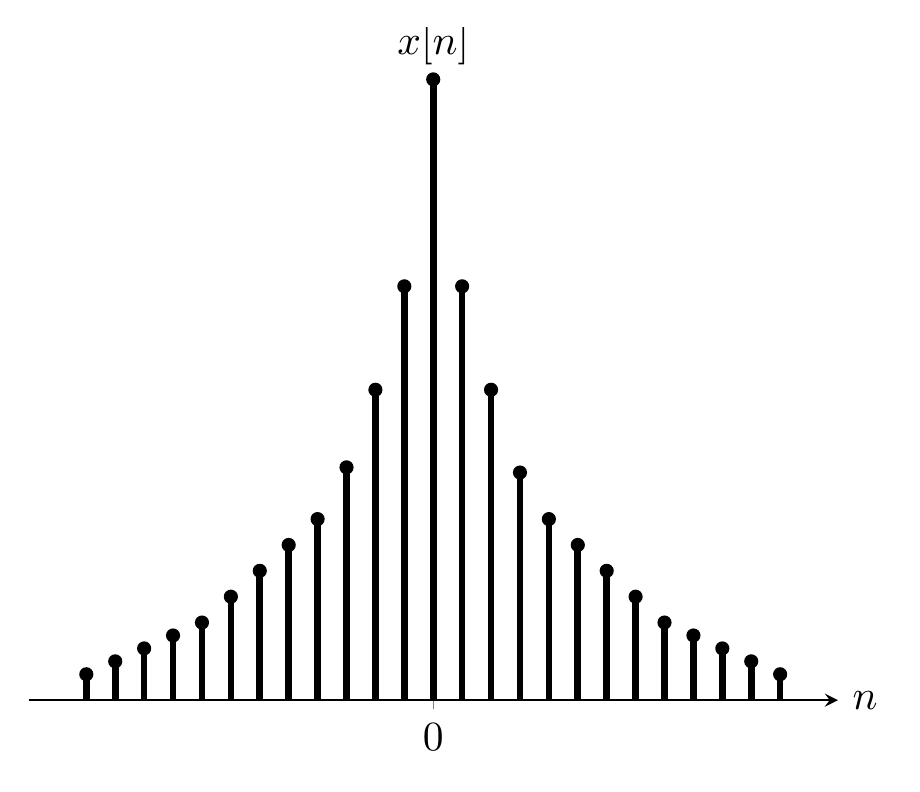
\begin{tikzpicture}[scale=1.5]
    \begin{axis}[
        axis x line=middle,
        axis y line=none,
        xmin=-14,xmax=14,
        ymin=0,ymax=13,
        xlabel=$n$,
        xlabel style = {anchor=west},
        xtick={0}
      ]
      info{
      \node at (0,12) [anchor=south] {$x[n]$};
      };
      \foreach\x/\y in {0/12,-1/8,1/8,2/6,-2/6,3/4.4,-3/4.5,4/3.5,-4/3.5,5/3,-5/3,6/2.5,-6/2.5,7/2,-7/2,8/1.5,-8/1.5,9/1.25,-9/1.25,10/1,-10/1,11/0.75,-11/0.75,12/0.5,-12/0.5}{
        \addplot[ultra thick,black,mark=none,] coordinates {(\x,0) (\x,\y)};
         \edef\temp{\noexpand\node at (\x,\y) [black node]{}; } \temp
         }
    \end{axis}
  \end{tikzpicture}
  }
  \newcommand{\answergraph}{
    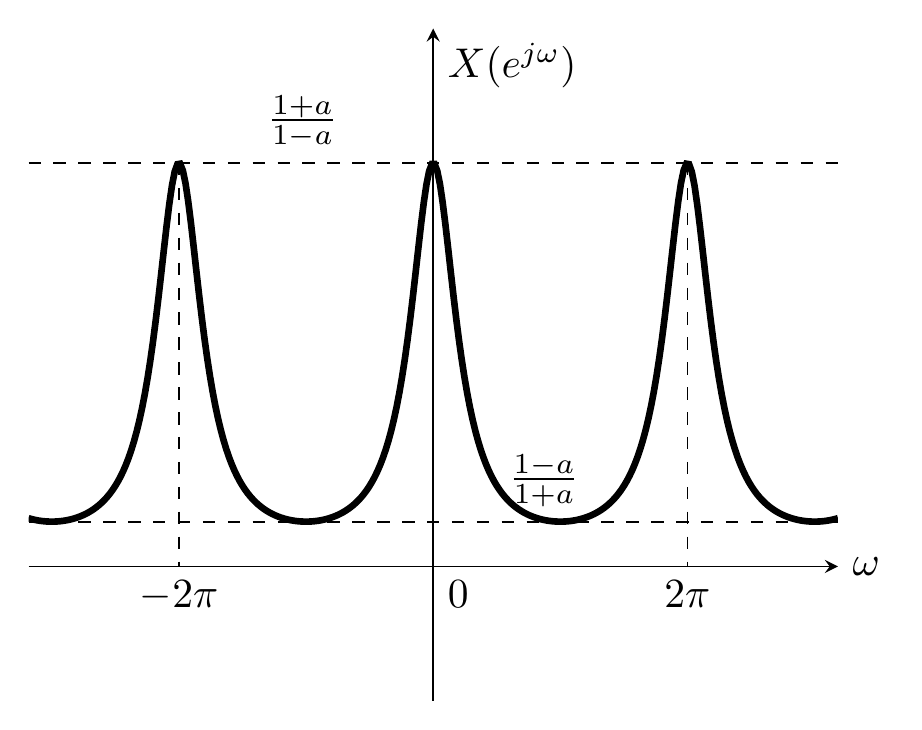
\begin{tikzpicture}[scale=1.5]
    \begin{axis}[
        axis x line=middle,
        axis y line=middle,
        xmin=-10 ,xmax=10,
        ymin=-1,ymax=4,
        xlabel=$\omega$,
        ylabel=$X(e^{j\omega})$,
        xlabel style = {anchor=south},
        xlabel style = {anchor=west},
        xtick={0},
        ytick={0},
        declare function = {
      s(\x) = (1-0.5*0.5)/(1-cos(deg(\x))+0.5*0.5);
    },
      ]
      info{
      \node at (0,0) [anchor=north west] {$0$};
      \node at (6.28,0) [anchor=north] {$2\pi$};
      \node at (-6.28,0) [anchor=north] {$-2\pi$};
      \node at (-2,3) [anchor=south east] {$\frac{1+a}{1-a}$};
      \node at (1.5,0.33) [anchor=south west] {$\frac{1-a}{1+a}$};
      };
      \addplot[domain=-10:10, samples=300,ultra thick, black] {s(x)};
      \addplot[dashed] coordinates {(-10,0.33) (10,0.33)};
      \addplot[dashed] coordinates {(-10,3) (10,3)};
      \addplot[dashed] coordinates {(-6.28,3) (-6.28,0)};
      \addplot[dashed] coordinates {(6.28,3) (6.28,0)};
    \end{axis}
  \end{tikzpicture}
  }
  \newcommand{\lowpass}{
    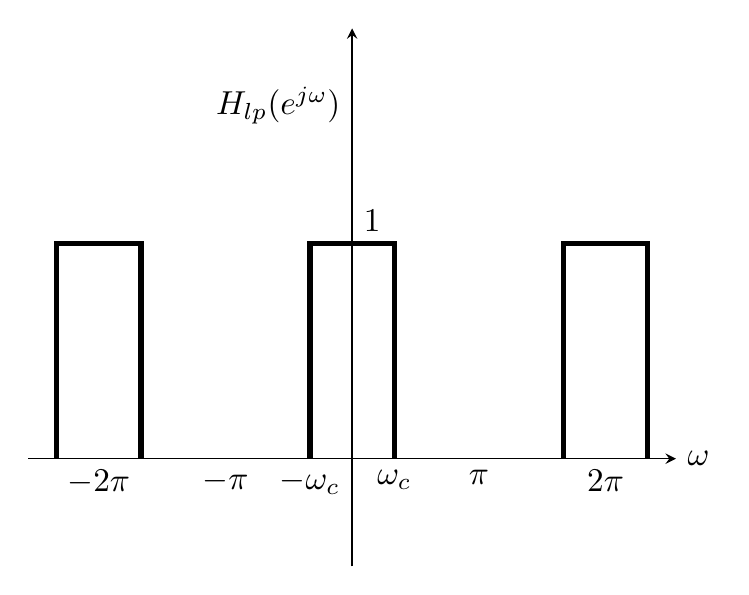
\begin{tikzpicture}[scale=1.2]
    \begin{axis}[
        axis x line=middle,
        axis y line=middle,
        xmin=-5.75,xmax=5.75,
        ymin=-0.5,ymax=2,
        xlabel=$\omega$,
        xlabel style = {anchor=west},
        xtick={0},
        ytick={0}
      ]
      info{
      \node at (0,1.5) [anchor=south east] {$H_{lp}(e^{j\omega})$};
      \node at (0,1) [anchor=south west] {$1$};
    \node at (-0.75,0) [anchor=north] {$-\omega_c$};
    \node at (0.75,0) [anchor=north] {$\omega_c$};
    \node at (-2.25,0) [anchor=north] {$-\pi$};
    \node at (2.25,0) [anchor=north] {$\pi$};
    \node at (-4.5,0) [anchor=north] {$-2\pi$};
    \node at (4.5,0) [anchor=north] {$2\pi$};
      };
      \addplot+[ultra thick, mark=none, black]  coordinates {(-0.75,0)(-0.75,1)(0.75,1)(0.75,0)};
      \addplot+[ultra thick, mark=none, black]  coordinates {(5.25,0)(5.25,1)(3.75,1)(3.75,0)};
      \addplot+[ultra thick, mark=none, black]  coordinates {(-5.25,0)(-5.25,1)(-3.75,1)(-3.75,0)};
         \end{axis}
  \end{tikzpicture}
  }
  \newcommand{\highpass}{
    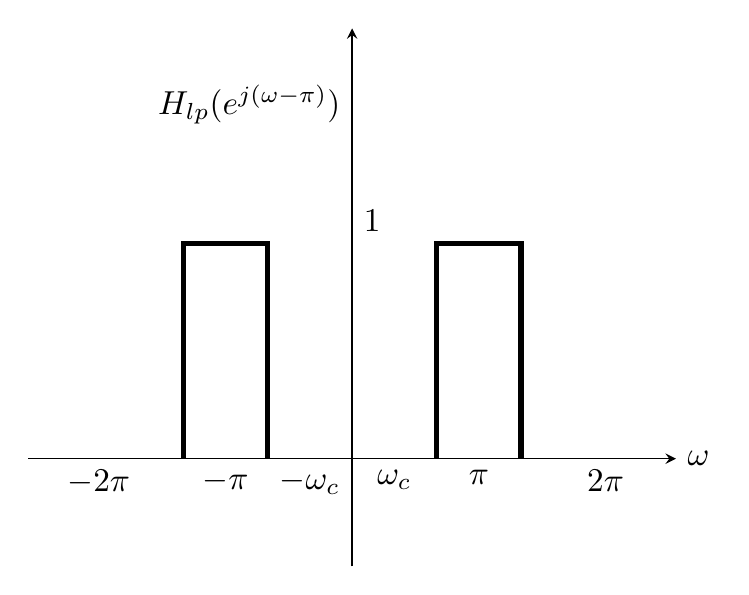
\begin{tikzpicture}[scale=1.2]
    \begin{axis}[
        axis x line=middle,
        axis y line=middle,
        xmin=-5.75,xmax=5.75,
        ymin=-0.5,ymax=2,
        xlabel=$\omega$,
        xlabel style = {anchor=west},
        xtick={0},
        ytick={0}
      ]
      info{
      \node at (0,1.5) [anchor=south east] {$H_{lp}(e^{j(\omega-\pi)})$};
      \node at (0,1) [anchor=south west] {$1$};
    \node at (-0.75,0) [anchor=north] {$-\omega_c$};
    \node at (0.75,0) [anchor=north] {$\omega_c$};
    \node at (-2.25,0) [anchor=north] {$-\pi$};
    \node at (2.25,0) [anchor=north] {$\pi$};
    \node at (-4.5,0) [anchor=north] {$-2\pi$};
    \node at (4.5,0) [anchor=north] {$2\pi$};
      };
      \addplot+[ultra thick, mark=none, black]  coordinates {(-3,0)(-3,1)(-1.5,1)(-1.5,0)};
      \addplot+[ultra thick, mark=none, black]  coordinates {(3,0)(3,1)(1.5,1)(1.5,0)};
         \end{axis}
  \end{tikzpicture}
  }
  \newtheorem{theorem}{Property}
\newtheorem{subtheorem}{Symmetry Property}[theorem]
\begin{document}
    \titlePage{Signal Analysis Assignment \#7}{November 23, 2020}{Dr. Dibakar Raj Panta}
    \problem{Find the DTFT of the signal $x[n]=a^{|n|}, |a|<1$}
    \solution{The signal $x[n]=a^{|n|}$ can be sketched for the range $0<a<1$ as in Figure~\ref{fig:question1}
    \begin{figure}[H]
        \centering
        \questiongraph
        \caption{Signal $x[n]=a^{|n|}$}
        \label{fig:question1}
        \end{figure}
        Using the standard formula for the Discrete Time Fourier Transform of a signal to find the DTFT of signal $x[n]$ as,
        \begin{equation*}
            \begin{aligned}
                X(e^{j\omega})&=\sum_{n=-\infty}^{\infty}a^{|n|}e^{-j\omega n}\\
                &=\sum_{n=0}^{\infty}a^{n}e^{-j\omega n}+\sum_{n=-\infty}^{-1}a^{-n}e^{-j\omega n}
            \end{aligned}
        \end{equation*}
        Changing the variable on the second term on R.H.S as $m=-n$,
        \begin{equation*}
            X(e^{j\omega})=\sum_{n=0}^{\infty}(ae^{-j\omega})^{n}+\sum_{m=1}^{\infty}(ae^{j\omega})^{m}
        \end{equation*}
        Expanding these summations as the infinite geometric series in closed form, we get,
        \begin{equation*}
            \begin{aligned}
                X(e^{j\omega})&=\frac{1}{1-ae^{-j\omega}}+\frac{ae^{j\omega}}{1-ae^{j\omega}}\\
                &=\frac{1-a^2}{1-2acos\omega +a^2}
            \end{aligned}
        \end{equation*}
        This equation represents the fourier transform of the signal $x[n]$. Figure~\ref{fig:answer1} shows the plot for $ X(e^{j\omega})$ since it is a real term as shown by the equation.
        \begin{figure}[H]
            \centering
            \answergraph
            \caption{Fourier Transform for signal shown in Figure~\ref{fig:question1} such that $0<a<1$}
            \label{fig:answer1}
            \end{figure}
    }
    \problem{Prove whether the system $y[n]=x[n]sin(\omega_0 n)$ is time variant or not.}
    \solution{The given system has an input of $x[n]$ and output $y[n]$. To check if the system is time variant or time invariant, we perform two sets of delays as,
    \subsubsection*{Delay the input}
    The system is fed with an input after delaying $x[n]$ by $n_0$. The output in this case would be,
    \begin{equation*}
        y_1[n]=x[n-n_0]sin(\omega_0 n)
    \end{equation*}
    \subsubsection*{Delay the output}
    The output $y[n]$ is delayed by $n_0$ after the unaltered input $x[n]$ is fed into the system. The output in this case would be,
    \begin{equation*}
        y_2[n]=y[n-n_0]=x[n-n_0]sin(\omega_0 n-\omega_0 n_0)
    \end{equation*}
    The resuts suggest that the different sets of delays result in different outputs, which is why we can conclude that the system is time variant.
    }
\problem{State and prove DTFT properties.}
\solution{
If $\ft{x[n]}$ denotes the fourier transformation of $x[n]$ into its fourier coefficients such that,
\begin{equation}
\ft{x[n]}=X(e^{j\omega}),\quad \text{where}\quad X(e^{j\omega})=\sum_{n=-\infty}^{\infty}x[n]e^{-j\omega n}
\label{eqn:DTFT}
\end{equation}
\begin{theorem}[Linearity]
    If $\ft{x[n]}=X(e^{j\omega})$ and $\ft{y[n]}=Y(e^{j\omega})$, then
    \begin{equation*}
    \ft{Ax[n]+By[n]}=AX(e^{j\omega})+BY(e^{j\omega})
    \end{equation*}
    \end{theorem}
    \begin{proof}
    This can be proved based on the properties of a summation over a limit.
    \begin{equation*}
    \begin{aligned} 
    \ft{Ax[n]+By[n]} &=\sum_{n=-\infty}^{\infty}(Ax[n]+By[n]) e^{-j\omega n} \\ 
    &= \sum_{n=-\infty}^{\infty}Ax[n] e^{-j\omega n}+\sum_{n=-\infty}^{\infty}By[n] e^{-j\omega n} \\
    &= A\sum_{n=-\infty}^{\infty}x[n] e^{-j\omega n}+B\sum_{n=-\infty}^{\infty}y[n] e^{-j\omega n} \\
    &= AX(e^{j\omega})+BY(e^{j\omega})
    \end{aligned}
    \end{equation*}
    \end{proof}
    \begin{theorem}[Time Shift]
        If $\ft{x[n]}=X(e^{j\omega})$ then
        \begin{equation*}
        \ft{x[n-n_0]}=e^{-j\omega n_0}X(e^{j\omega})
        \end{equation*}
        \end{theorem}
        \begin{proof}
        \begin{equation*}
        \begin{aligned} 
        \ft{x[n-n_0]} &=\sum_{n=-\infty}^{\infty} x[n-n_0] e^{-j\omega n} \\ 
        &=\sum_{m=-\infty}^{\infty} x[m] e^{-j\omega (m+n_0)} \quad \text{where,}\quad m=n-n_0\\
        &=\sum_{m=-\infty}^{\infty} x[m] e^{-j\omega m}e^{-j\omega n_0} \\
        &=e^{-j\omega n_0}\sum_{m=-\infty}^{\infty} x[m] e^{-j\omega m}\\
        &=e^{-j\omega n_0}X(e^{j\omega})
        \end{aligned}
        \end{equation*}
        \end{proof}
        \begin{theorem}[Frequency Shift]
            If $\ft{x[n]}=X(e^{j\omega})$ then
            \begin{equation*}
            \ft{e^{j\omega_0 n} x[n]}=X(e^{j(\omega-\omega_0)})
            \end{equation*}
            \end{theorem}
            \begin{proof}
            \begin{equation*}
            \begin{aligned} 
            \ft{e^{j\omega_0 n} x[n]} &=\sum_{n=-\infty}^{\infty} e^{j\omega_0 n} x[n] e^{-j\omega n} \\
            &=\sum_{n=-\infty}^{\infty} x[n] e^{-j(\omega-\omega_0)n}\\
            &=X(e^{j(\omega-\omega_0)})
            \end{aligned}
            \end{equation*}
            \end{proof}
            \begin{theorem}[Time Scaling(Expansion)]
                If $\ft{x[n]}=\begin{cases}
                    x[n/k] \quad \text{if n/k is an integer}\\
                    0 \quad otherwise
                \end{cases}$ then
                \begin{equation*}
                \ft{x[n]}=X(e^{jk\omega})
                \end{equation*}
                \end{theorem}
                \begin{proof}
                The DTFT time scaling property is available only for expansion in the time domain. This is because decimation discards samples of the original signal and therefore there is no unique relationship between the original signal and a decimated signal.
                \begin{equation*}
                \begin{aligned} 
                \ft{x[n]} &=\sum_{n=-\infty}^{\infty} x[n/k] e^{-j\omega n} \\
                &=\sum_{m=-\infty}^{\infty} x[m] e^{-j\omega km} \quad \text{where,}\quad m=n/k\\
                &=X(e^{jk\omega})
                \end{aligned}
                \end{equation*}
                \end{proof}
                \begin{theorem}[Differentiation in Frequency Domain]
                    If $\ft{x[n]}=X(e^{j\omega})$ then
                    \begin{equation*}
                    \ft{nx[n]}=j\frac{dX(e^{j\omega})}{d\omega}
                    \end{equation*}
                    \end{theorem}
                    \begin{proof}
                    \begin{equation*}
                    \begin{aligned} 
                    X(e^{j\omega})&=\sum_{n=-\infty}^{\infty} x[n] e^{-j\omega n} \\
                    j X(e^{j\omega})&=j\sum_{n=-\infty}^{\infty} x[n] e^{-j\omega n}\\
                    j\frac{dX(e^{j\omega})}{d\omega}&=j\sum_{n=-\infty}^{\infty} x[n] \frac{de^{-j\omega n}}{d\omega}\\
                    j\frac{dX(e^{j\omega})}{d\omega}&=j.(-j)\sum_{n=-\infty}^{\infty} nx[n] e^{-j\omega n}\\
                    j\frac{dX(e^{j\omega})}{d\omega}&=\sum_{n=-\infty}^{\infty} nx[n] e^{-j\omega n}=\ft{nx[n]}\\
                    \end{aligned}
                    \end{equation*}
                    \end{proof}
                    \begin{theorem}[Differencing in Time Domain]
                        If $\ft{x[n]}=X(e^{j\omega})$ then
                        \begin{equation*}
                        \ft{x[n]-x[n-1]}=(1-e^{-j\omega})X(e^{j\omega})
                        \end{equation*}
                        \end{theorem}
                        \begin{proof}This can be proved by using the linearity and time shifting properties mentioned above.
                        \begin{equation*}
                        \begin{aligned} 
                            \ft{x[n]-x[n-1]}&=\ft{x[n]}-\ft{x[n-1]}\\
                            &=X(e^{j\omega})-e^{-j\omega}X(e^{j\omega})\\
                            &=(1-e^{-j\omega})X(e^{j\omega})
                        \end{aligned}
                        \end{equation*}
                        \end{proof}
                        \begin{theorem}[Time Reversal]
                            If $\ft{x[n]}=X(e^{j\omega})$ then
                            \begin{equation*}
                            \ft{x[-n]}=X(e^{-j\omega})
                            \end{equation*}
                            \end{theorem}
                            \begin{proof}
                            \begin{equation*}
                            \begin{aligned} 
                            \ft{x[-n]}&=\sum_{n=-\infty}^{\infty} x[-n] e^{-j\omega n} \\
                            &=\sum_{m=-\infty}^{\infty} x[m] e^{-j(-\omega) m} \quad \text{where,}\quad m=-n\\
                            &=X(e^{-j\omega})
                            \end{aligned}
                            \end{equation*}
                            \end{proof}
                        \begin{theorem}[Multiplication]
    If $\ft{x[n]}=X(e^{j\omega})$ and $\ft{y[n]}=Y(e^{j\omega})$, then
    \begin{equation*}
    \ft{x[n]y[n]}=\frac{1}{2\pi}[X(e^{j\omega})*Y(e^{j\omega})]
    \end{equation*}
    \end{theorem}
    \begin{proof}Using the definition of IDTFT,
    \begin{equation*}
    \begin{aligned} 
        x[n]=\frac{1}{2\pi}\int_{2\pi}X(e^{j\omega})e^{j\omega n} d\omega\\
        x[n]=\frac{1}{2\pi}\int_{2\pi}X(e^{j\theta})e^{j\theta n} d\theta\\
    \end{aligned}
    \end{equation*}
    Using Equation~\ref{eqn:DTFT} for the signal $x[n]y[n]$,
    \begin{equation*}
        \begin{aligned} 
           \ft{x[n]y[n]}&=\sum_{n=-\infty}^{\infty} x[n]y[n] e^{-j\omega n}\\
           &=\sum_{n=-\infty}^{\infty} \left(\frac{1}{2\pi}\int_{2\pi}X(e^{j\theta})e^{j\theta n} d\theta\right)y[n] e^{-j\omega n}\\
           &=\frac{1}{2\pi}\int_{2\pi}X(e^{j\theta})\sum_{n=-\infty}^{\infty}y[n] e^{-j(\omega-\theta) n} d\theta\\
           &=\frac{1}{2\pi}\int_{2\pi}X(e^{j\theta})Y(e^{j(\omega-\theta})d\theta\\
           &=\frac{1}{2\pi}[X(e^{j\omega})*Y(e^{j\omega})]
        \end{aligned}
        \end{equation*}
    \end{proof}
    \begin{theorem}[Conjugation]
        If $\ft{x[n]}=X(e^{j\omega})$ then
        \begin{equation*}
        \ft{x^*[n]}=X^*(e^{-j\omega})
        \end{equation*}
        \end{theorem}
        \begin{proof}
        \begin{equation*}
        \begin{aligned} 
            \ft{x^*[n]}&=\sum_{n=-\infty}^{\infty} x^*[n] e^{-j\omega n}\\
            &=\left(\sum_{n=-\infty}^{\infty} x[n] e^{j\omega n}\right)^*\\
            &=\left(\sum_{n=-\infty}^{\infty} x[n] e^{-j(-\omega) n}\right)^*\\
            &=X^*(e^{-j\omega})
        \end{aligned}
        \end{equation*}
        \end{proof}
        \begin{theorem}[Symmetry Properties]
            A signal $x[n]$ has various symmetry properties for odd, even and real valued conditions as,
            \end{theorem}
            \begin{subtheorem}[Conjugate Symmetry for real signal]
                If $\ft{x[n]}=X(e^{j\omega})$ such that $x[n]$ is a real signal then
                \begin{equation*}
                    X(e^{j\omega})=X^*(e^{-j\omega})
                \end{equation*}
                \end{subtheorem}
                \begin{proof}
                   For a real signal $x[n]$, the relation $x[n]=x^*[n]$ holds true. From the conjugation property mentioned above, we can write, $\ft{x^*[n]}=X^*(e^{-j\omega})$, so,
                   \begin{equation*}
                    \begin{aligned} 
                       x[n]&=x^*[n]\\
                       \ft{x[n]}&=\ft{x^*[n]}\\
                       X^(e^{j\omega})&=X^*(e^{-j\omega})
                    \end{aligned}
                    \end{equation*}
                    The following conclusions can be drawn from the conjugate symmetry property.
                    \begin{equation*}
                        \begin{aligned} 
                           \Re(X(e^{j\omega}))&=\Re(X(e^{-j\omega}))\\
                           \Im(X(e^{j\omega}))&=-\Im(X(e^{-j\omega}))\\
                           |X(e^{j\omega})|&=|X(e^{-j\omega})|\\
                           \measuredangle X(e^{j\omega})&=\measuredangle X(e^{-j\omega})
                        \end{aligned}
                        \end{equation*}
                \end{proof}
                \begin{subtheorem}[Real and even signal]
                For a real signal $x[n]$ such that $x[n]=x[-n]$,
                 the fourier transform $\ft{x[n]}=X(e^{j\omega})$ is real and even.
                    \end{subtheorem}
                    \begin{proof}
                       \begin{equation*}
                        \begin{aligned} 
                            \ft{x[n]}&=\sum_{n=-\infty}^{\infty} x[n] e^{-j\omega n}\\
                            &=\sum_{n=-\infty}^{\infty} x[n] (cos(\omega n)-jsin(\omega n))\\
                            &=\sum_{n=-\infty}^{\infty} x[n] cos(\omega n)-j \sum_{n=-\infty}^{\infty} x[n]sin(\omega n)\\
                            X(e^{j\omega})&=\sum_{n=-\infty}^{\infty} x[n] cos(\omega n)
                        \end{aligned}
                        \end{equation*}
                        The above result indicates that the fourier transform of a real and even signal is indeed real and even. This is true since the product of an even signal $x[n]$ and an odd signal $sin(\omega n)$ is odd and the summation of an odd signal is 0, which reduces the entire imaginary term into 0. The remaining summation is even and real.
                    \end{proof}
                    \begin{subtheorem}[Real and odd signal]
                        For a real signal $x[n]$ such that $x[n]=-x[-n]$,
                         the fourier transform $\ft{x[n]}=X(e^{j\omega})$ is purely imaginary and odd.
                            \end{subtheorem}
                            \begin{proof}
                               \begin{equation*}
                                \begin{aligned} 
                                    \ft{x[n]}&=\sum_{n=-\infty}^{\infty} x[n] e^{-j\omega n}\\
                                    &=\sum_{n=-\infty}^{\infty} x[n] (cos(\omega n)-jsin(\omega n))\\
                                    &=\sum_{n=-\infty}^{\infty} x[n] cos(\omega n)-j \sum_{n=-\infty}^{\infty} x[n]sin(\omega n)\\
                                    X(e^{j\omega})&=-j \sum_{n=-\infty}^{\infty} x[n]sin(\omega n)
                                \end{aligned}
                                \end{equation*}
                                The above result indicates that the fourier transform of a real and odd signal is indeed purely imaginaru and odd. This is true since the product of an odd signal $x[n]$ and an even signal $cos(\omega n)$ is odd and the summation of an odd signal is 0, which reduces the entire real term into 0. The remaining summation is  odd and purely imaginary.
                            \end{proof}
        \begin{theorem}[Convolution]
            If $\ft{x[n]}=X(e^{j\omega})$ and $\ft{y[n]}=Y(e^{j\omega})$, then
            \begin{equation*}
            \ft{x[n]*y[n]}=X(e^{j\omega})Y(e^{j\omega})
            \end{equation*}
            \end{theorem}
            \begin{proof}
            \begin{equation*}
                \begin{aligned} 
                   \ft{x[n]*y[n]}&=\sum_{n=-\infty}^{\infty} (x[n]*y[n]) e^{-j\omega n}\\
                   &=\sum_{n=-\infty}^{\infty} \sum_{k=-\infty}^{\infty} x[k]y[n-k] e^{-j\omega n}\\
                   &=\sum_{k=-\infty}^{\infty} x[k] \sum_{n=-\infty}^{\infty} y[n-k] e^{-j\omega n}\\
                   &=\sum_{k=-\infty}^{\infty} x[k] \sum_{m=-\infty}^{\infty} y[m] e^{-j\omega (m+k)}\quad \text{where,}\quad m=n-k\\
                   &=\sum_{k=-\infty}^{\infty} x[k] e^{-j\omega k} \sum_{m=-\infty}^{\infty} y[m] e^{-j\omega m} \\
                   &=X(e^{j\omega})Y(e^{j\omega})
                \end{aligned}
                \end{equation*}
            \end{proof}
            \begin{theorem}[Parseval's Relation]
                If $\ft{x[n]}=X(e^{j\omega})$ then
                \begin{equation*}
                    \sum_{n=-\infty}^{\infty} |x[n]|^2=\frac{1}{2\pi}\int_{-\pi}^{\pi}|X(e^{j\omega})|^2 d\omega
                \end{equation*}
                \end{theorem}
                \begin{proof}
                    Using the definition of IDTFT,
                    \begin{equation*}
                        \begin{aligned} 
                            x[n]&=\frac{1}{2\pi}\int_{-\pi}^{\pi}X(e^{j\omega})e^{j\omega n} d\omega \quad \text{and,}\\
                            x^*[n]&=\frac{1}{2\pi}\int_{-\pi}^{\pi}X^*(e^{j\omega})e^{-j\omega n} d\omega
                        \end{aligned}
                        \end{equation*}
                So,
                \begin{equation*}
                    \begin{aligned} 
                        \sum_{n=-\infty}^{\infty} |x[n]|^2&=\sum_{n=-\infty}^{\infty} x[n]x^*[n]\\
                        &=\sum_{n=-\infty}^{\infty} x[n] \frac{1}{2\pi}\int_{-\pi}^{\pi}X^*(e^{j\omega})e^{-j\omega n} d\omega\\
                        &=\frac{1}{2\pi}\int_{-\pi}^{\pi}X^*(e^{j\omega})\sum_{n=-\infty}^{\infty} x[n]e^{-j\omega n} d\omega\\
                        &=\frac{1}{2\pi}\int_{-\pi}^{\pi}X^*(e^{j\omega})X(e^{j\omega})d\omega\\
                        &=\frac{1}{2\pi}\int_{-\pi}^{\pi}|X(e^{j\omega})|^2 d\omega
                    \end{aligned}
                    \end{equation*}
                \end{proof}
}
\problem{Discuss the relationship between ideal low pass and ideal high pass discrete-time filters based on the periodicity and frequency shifting properties of DTFT. (Example 5.7 from Signals \& Systems by Alan V. Oppenheim)}
\solution{
    The frequency response, $H_{lp}(e^{j\omega})$, for a lowpass filter with $\omega_c$ as the cutoff frequency is plotted in Figure~\ref{fig:lowpass}. Plot for another frequency response $H_{lp}(e^{j(\omega-\pi)})$, which is shifted by one-half period i.e. $\pi$, is shown in Figure~\ref{fig:highpass}. The frequency response $H_{lp}(e^{j(\omega-\pi)})$ is that of an ideal highpass filter with cutoff frequency as $\pi-\omega_c$ since the frequencies in discrete time are concentrated near odd multiples of $\pi$. Mathematically,
    \begin{equation*}
       H_{hp}(e^{j\omega})=H_{lp}(e^{j(\omega-\pi)})
    \end{equation*}
    \begin{figure}[H]
        \centering
        \lowpass
        \caption{Frequency response of a lowpass filter}
        \label{fig:lowpass}
    \end{figure}
    \begin{figure}[H]
        \centering
        \highpass
        \caption{Frequency response of a highpass filter obtained by shifting the frequency response in Figure~\ref{fig:lowpass} by $\omega=\pi$ corresponding to one half period}
        \label{fig:highpass}
    \end{figure}
    The frequency response of an LTI system is the fourier transform of the system's impulse response. Mathematically,
    \begin{equation*}
        H(e^{j\omega})=\sum_{n=-\infty}^{\infty}h[n]e^{-j\omega n}
     \end{equation*}
     So, if the impulse responses of the two filters shown in Figure~\ref{fig:lowpass} and \ref{fig:highpass} are $h_{lp}[n]$ and $h_{hp}[n]$, then by using the frequency shift property of DTFT, we can conclude with a relation between the two impulse responses as,
     \begin{equation*}
         \begin{aligned}
            h_{hp}[n]&=e^{j\pi n}h_{lp}[n]\\
            &=(-1)^n h_{lp}[n]
         \end{aligned}
     \end{equation*}
}
\end{document}